\documentclass{article}

\usepackage{geometry}
\usepackage{longtable}
\usepackage[dvipsnames,table]{xcolor}
\usepackage{fancyhdr}
\usepackage{xcolor}
\usepackage{graphicx}
\usepackage{hyperref}
\usepackage{float}
\usepackage{listings}
\usepackage{amssymb}
\usepackage{amsmath}
\usepackage{enumitem}
\usepackage{parskip}

% Choose paper size
\geometry{letterpaper, top=25.4mm, bottom=25.4mm, left=25.4mm, right=25.4mm}

\color{black}
\fancyhf{}
\renewcommand{\headrulewidth}{1pt}
\renewcommand{\footrulewidth}{1pt}

% Define standard IPF color palette
\definecolor{soft-sky-blue}{HTML}{B7DAEB}
\definecolor{orange}{HTML}{FF6633}
\definecolor{cool-grey}{HTML}{91A1B0}
\definecolor{black}{HTML}{000000}
\definecolor{space-blue}{HTML}{003366}
\definecolor{pigeon-blue}{HTML}{5F8396}
\definecolor{sage-green}{HTML}{95A077}
\definecolor{fire-yellow}{HTML}{F9A651}
\definecolor{apple-red}{HTML}{CC4200}
\definecolor{crockadile-green}{HTML}{718944}
\definecolor{slate-grey}{HTML}{607587}
\definecolor{fog-grey}{HTML}{E5E6E9}

% Define certification colors
\definecolor{cert-level-0}{HTML}{CC4200} % apple-red
\definecolor{cert-level-1}{HTML}{FF6633} % orange
\definecolor{cert-level-2}{HTML}{F9A651} % fire-yellow
\definecolor{cert-level-3}{HTML}{B7DAEB} % soft-sky-blue
\definecolor{cert-level-4}{HTML}{5F8396} % pigeon-blue
\definecolor{cert-level-5}{HTML}{718944} % sage-green

\hypersetup{hidelinks}
\pagestyle{fancy}
\pagenumbering{arabic}

\title{

\includegraphics[width=8cm] {images/Rocksavage_Tech_RGB_300.png}\vspace{50pt}
\vspace{10pt} \\
\textbf{Timer \\
  Product User Guide} \\
{\small{\textcolor{slate-grey}{rocksavagetech.chiselWare.Timer}}} \\
\vspace{20pt} IPF certified to level:
\textbf{\textcolor{cert-level-0}{0} }of 5 \\
\vspace{5pt}

\includegraphics[width=4cm] {images/uncertified.png}
}

\author{Warren Savage}

\fancyhead[L]{Timer Users Guide}
\fancyhead[R]{\leftmark}
\fancyfoot[C]{Rocksavage Technology, Inc.~\copyright~2023}
\fancyfoot[R]{Page \thepage}

\begin{document}

\maketitle
\newpage
\tableofcontents

\section{Errata and Known Issues}

\subsection{Errata}
\begin{itemize}
    \item It should be noted that the baud rate is set by an interative divider. It can take up to 32 clock cycles to converge to a division result.
\end{itemize}

\subsection{Known Issues}
None.
\section{Port Descriptions}

The UART module provides two sets of ports:
\begin{enumerate}
  \item The external UART interface (serial TX and RX signals)
  \item The APB interface for register access
\end{enumerate}

\subsection{UART Interface}

The UART-specific ports allow the module to communicate with external devices over a standard asynchronous serial link. The key signals are:

\renewcommand*{\arraystretch}{1.3}
\begingroup
\small
\rowcolors{2}{gray!30}{gray!10}
\begin{longtable}[H]{
  | p{0.25\textwidth}
  | p{0.15\textwidth}
  | p{0.15\textwidth}
  | p{0.40\textwidth} |
}
\hline
\rowcolor{gray}
\textcolor{white}{\textbf{Port Name}} &
\textcolor{white}{\textbf{Width}} &
\textcolor{white}{\textbf{Direction}} &
\textcolor{white}{\textbf{Description}} \\ \hline
\endfirsthead

\hline
\rowcolor{gray}
\textcolor{white}{\textbf{Port Name}} &
\textcolor{white}{\textbf{Width}} &
\textcolor{white}{\textbf{Direction}} &
\textcolor{white}{\textbf{Description}} \\ \hline
\endhead

\hline
\endfoot

\texttt{rx} &
1 &
Input &
Asynchronous serial receive data input. This signal is synchronized internally and sampled by the receiver FSM. \\ \hline

\texttt{tx} &
1 &
Output &
Serial transmit data output. When idle, this line remains high. \\ \hline
\end{longtable}
\captionof{table}{UART Interface Ports}
\label{table:uart_ports}
\endgroup

\subsection{APB Interface}

The APB interface provides access to the UART’s registers, allowing software to configure and monitor both the TX and RX operations (including baud rate settings, FIFO control, and error status). The APB signals are defined as follows:

\renewcommand*{\arraystretch}{1.3}
\begingroup
\small
\rowcolors{2}{gray!30}{gray!10}
\begin{longtable}[H]{
  | p{0.20\textwidth}
  | p{0.20\textwidth}
  | p{0.12\textwidth}
  | p{0.43\textwidth} |
}
\hline
\rowcolor{gray}
\textcolor{white}{\textbf{Port Name}} &
\textcolor{white}{\textbf{Width}} &
\textcolor{white}{\textbf{Direction}} &
\textcolor{white}{\textbf{Description}} \\ \hline
\endfirsthead

\hline
\rowcolor{gray}
\textcolor{white}{\textbf{Port Name}} &
\textcolor{white}{\textbf{Width}} &
\textcolor{white}{\textbf{Direction}} &
\textcolor{white}{\textbf{Description}}\\ \hline
\endhead

\hline
\endfoot

\texttt{PCLK} &
1 &
Input &
APB clock signal for register access. \\ \hline

\texttt{PRESETN} &
1 &
Input &
Active–low asynchronous reset. \\ \hline

\texttt{PSEL} &
1 &
Input &
Select signal indicating that the UART is addressed. \\ \hline

\texttt{PENABLE} &
1 &
Input &
Indicates the second cycle of an APB transfer. \\ \hline

\texttt{PWRITE} &
1 &
Input &
Determines the operation: HIGH for write, LOW for read. \\ \hline

\texttt{PADDR} &
\textit{addressWidth} &
Input &
APB address bus for register selection. \\ \hline

\texttt{PWDATA} &
\textit{dataWidth} &
Input &
APB write data bus. \\ \hline

\texttt{PRDATA} &
\textit{dataWidth} &
Output &
APB read data bus. \\ \hline

\texttt{PREADY} &
1 &
Output &
Indicates that the UART is ready for the next transfer. \\ \hline

\texttt{PSLVERR} &
1 &
Output &
Indicates a transfer error. \\ \hline
\end{longtable}
\captionof{table}{APB Interface Ports}
\label{table:apb_ports}
\endgroup

\section{Parameter Descriptions}

Table~\ref{table:params} summarizes the key parameters for the \textbf{UART} module. Each can be customized during instantiation.

\renewcommand*{\arraystretch}{1.3}
\begingroup
\small
\rowcolors{2}{gray!30}{gray!10}
\arrayrulecolor{gray!80}

\begin{longtable}[H]{
  | p{0.22\textwidth}
  | p{0.13\textwidth}
  | p{0.08\textwidth}
  | p{0.08\textwidth}
  | p{0.42\textwidth} |
}
\hline
\rowcolor{gray}
\textcolor{white}{\textbf{Name}} &
\textcolor{white}{\textbf{Type}} &
\textcolor{white}{\textbf{Min}} &
\textcolor{white}{\textbf{Max}} &
\textcolor{white}{\textbf{Description}} \\ 
\hline
\endfirsthead

\hline
\rowcolor{gray}
\textcolor{white}{\textbf{Name}} &
\textcolor{white}{\textbf{Type}} &
\textcolor{white}{\textbf{Min}} &
\textcolor{white}{\textbf{Max}} &
\textcolor{white}{\textbf{Description}} \\ 
\hline
\endhead

\hline
\endfoot

\texttt{dataWidth} &
Integer &
8 &
32 &
Data width for APB bus operations. \\ \hline

\texttt{addressWidth} &
Integer &
1 &
-- &
Address width for APB bus. \\ \hline

\texttt{maxClocksPerBit} &
Integer &
2 &
-- &
Maximum allowed clock cycles per UART bit. Determines maximum baud rate. \\ \hline

\texttt{maxOutputBits} &
Integer &
5 &
16 &
Maximum number of data bits plus optional parity bit. Typically up to 9 or so, here parameterized. \\ \hline

\texttt{fifoDepth} &
Integer &
1 &
-- &
Depth of the internal RX/TX FIFOs. Must be a power of 2. \\ \hline

\texttt{syncDepth} &
Integer &
2 &
-- &
Depth for RX input synchronization. Recommended at least 2 for metastability protection. \\ \hline

\texttt{parity} &
Bool &
N/A &
N/A &
Default parity selection (odd/even). This can be overridden by registers at runtime. \\ \hline

\texttt{verbose} &
Bool &
N/A &
N/A &
Enables debugging \texttt{printf} statements. \\ \hline

\end{longtable}
\captionof{table}{UART Parameter Descriptions}
\label{table:params}
\endgroup

\noindent
A typical instantiation in Scala might look like:
\begin{lstlisting}[language=Scala]
// Example instantiation
val myUart = Module(new Uart(
  UartParams(
    dataWidth       = 32,
    addressWidth    = 32,
    maxClocksPerBit = 217,
    maxOutputBits   = 8,
    fifoDepth       = 16,
    syncDepth       = 2,
    parity          = false,
    verbose         = false
  ),
  formal = false
))
\end{lstlisting}

\section{Theory of Operations}

\subsection{Introduction}
The \textbf{Timer} is a configurable timer module that supports a variety of timing functions, including PWM generation and interrupt signaling. It features a counter that can be configured with a prescaler, maximum count value, and PWM ceiling value.

\begin{figure}[h]
  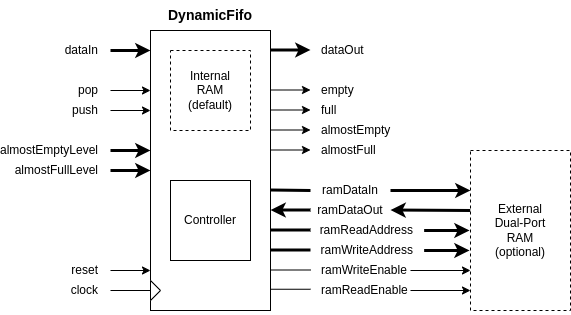
\includegraphics[width=0.80\textwidth]{images/block-diagram.png}
  \caption{Block Diagram}\label{fig:block-diagram}
\end{figure}

The Timer module provides the following outputs:

\begin{itemize}[noitemsep]
  \item{\textit{count}: Current value of the counter.}
  \item{\textit{maxReached}: Signal indicating the counter has reached its maximum value.}
  \item{\textit{pwm}: PWM output signal with a duty cycle controlled by \textit{pwmCeiling}.}
  \item{\textit{interrupt}: Interrupt signal indicating timer events (e.g., max reached).}
\end{itemize}

\subsection{Interface Timing}
The Timer operates on a synchronous clock and provides outputs that are valid on the rising edge of the clock. The timing diagram below illustrates the behavior of the Timer when the counter reaches its maximum value and generates an interrupt.

% \begin{figure}[h]
%   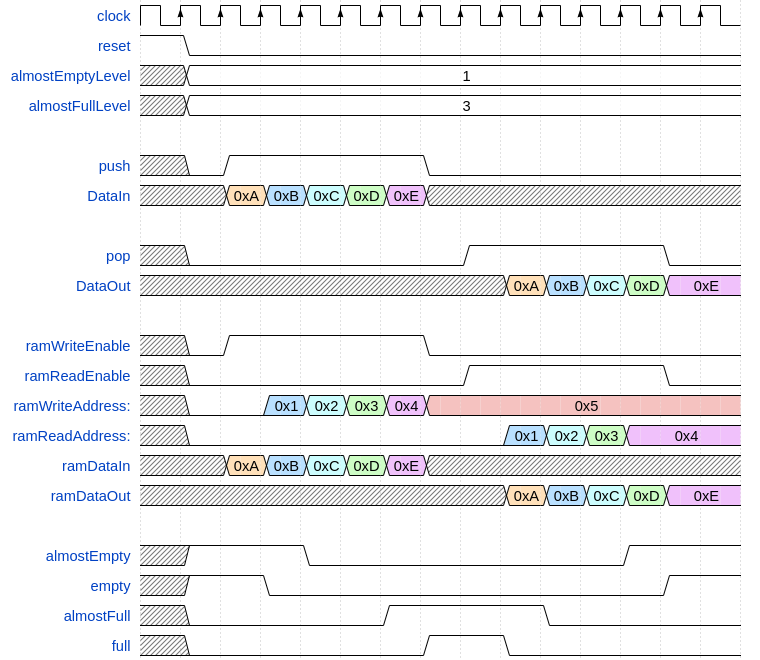
\includegraphics[width=\textwidth]{images/timing.png}
%   \caption{Timing Diagram}\label{fig:timing}
% \end{figure}
\section{Simulation}

\subsection{Tests}
The test bench for the Timer module includes directed tests that verify the functionality of the counter, PWM generation, and interrupt signaling. The tests cover the following scenarios:

\begin{itemize}
  \item{Basic counter operation with and without a prescaler.}
  \item{PWM generation with varying duty cycles.}
  \item{Interrupt generation when the counter reaches its maximum value.}
\end{itemize}

\subsection{Code Coverage}
All inputs and outputs are checked to ensure they toggle at least once during simulation. An error will be thrown if any port fails to toggle.

\subsection{Running Simulation}
Simulations can be run directly from the command prompt as follows:

\begin{verbatim}
  $ sbt "test"
\end{verbatim}

or from make as follows:

\texttt{\$ make test}
\section{Synthesis}

\subsection{Area and Gate Count}
Example synthesis results vary based on \texttt{fifoDepth} and other settings. An illustrative table:

\renewcommand*{\arraystretch}{1.3}
\begingroup
\small
\rowcolors{2}{gray!30}{gray!10}
\begin{longtable}[H]{
  | p{0.22\textwidth}
  | p{0.18\textwidth}
  | p{0.20\textwidth}
  | p{0.30\textwidth} |
}
\hline
\rowcolor{gray}
\textcolor{white}{\textbf{Config}} &
\textcolor{white}{\textbf{FIFO Depth}} &
\textcolor{white}{\textbf{Data Bits}} &
\textcolor{white}{\textbf{Gate Count}} \\ 
\hline
\endfirsthead

\hline
\rowcolor{gray}
\textcolor{white}{\textbf{Config}} &
\textcolor{white}{\textbf{FIFO Depth}} &
\textcolor{white}{\textbf{Data Bits}} &
\textcolor{white}{\textbf{Gate Count}} \\ 
\hline
\endhead

\hline
\endfoot

\texttt{uart\_8\_depth4}  & 4  & 8  & 2,200 gates \\ \hline
\texttt{uart\_8\_depth16} & 16 & 8  & 3,100 gates \\ \hline
\texttt{uart\_9\_depth16} & 16 & 9  & 3,400 gates \\ \hline

\caption{Example Synthesis Results}
\end{longtable}
\endgroup

\subsection{Timing Constraints}
An \texttt{.sdc} file can be generated to specify clock period, input/output constraints, etc. For example:
\begin{verbatim}
create_clock -name PCLK -period 10.0 [get_ports PCLK]
set_input_delay 2.0 -clock PCLK [get_ports rx]
set_output_delay 2.0 -clock PCLK [get_ports tx]
\end{verbatim}

\subsection{Multicycle and False Paths}
Typically, no multicycle or false paths are required if the design runs entirely from \texttt{PCLK} with no asynchronous logic. Check your usage and tool warnings for final closure.


\end{document}